\begin{titlepage}

\begin{figure}[H]
  \begin{center}
    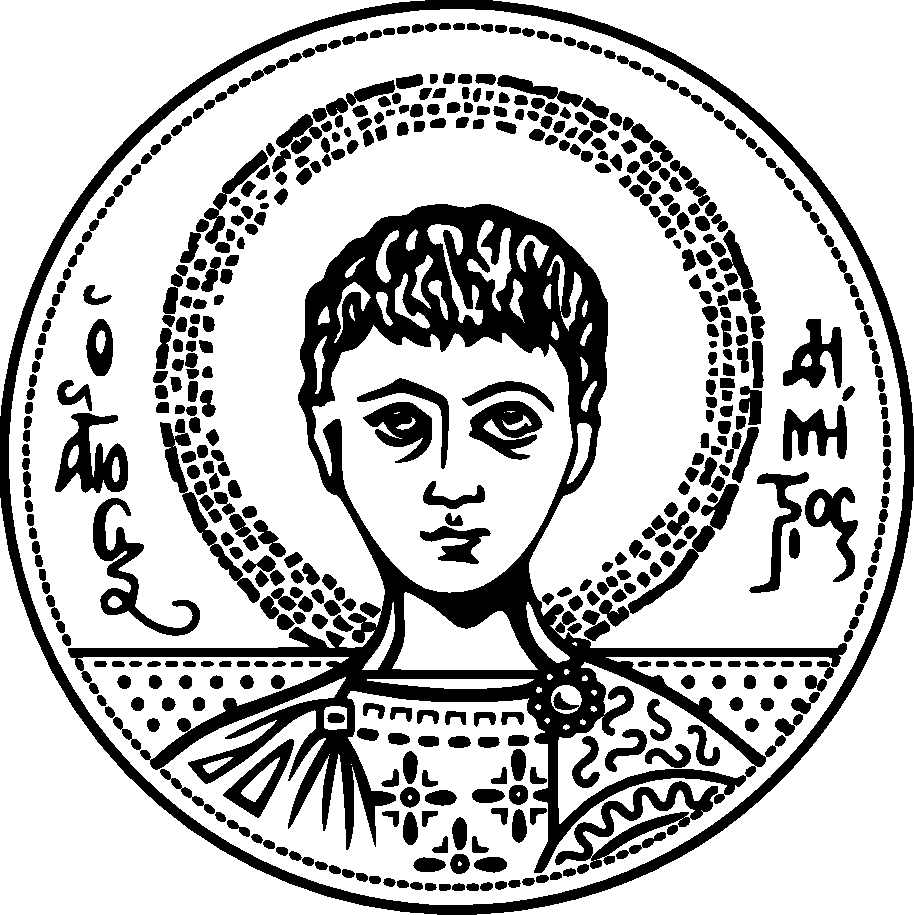
\includegraphics[width=3cm]{auth.pdf}
    \label{fig:cover_auth_logo}
  \end{center}
\end{figure}

\centering
\Large Αριστοτέλειο Πανεπιστήμιο Θεσσαλονίκης\\
\Large Πολυτεχνική Σχολή\\
\large Τμήμα Ηλεκτρολόγων Μηχανικών και Μηχανικών Υπολογιστών\\
\large Τομέας Ηλεκτρονικής και Υπολογιστών\\

\vspace{\fill}

\LARGE Αυτοεπιβλεπόμενη μάθηση με δεδομένα βίντεο για περιβάλλοντα με περιορισμένους υπολογιστικούς πόρους



\vspace{\fill}

\Large Διπλωματική Εργασία\\
\Large του\\
\Large Γεώργιου Ιωαννίδη\\

\vspace{\fill}
\raggedright

\begin{tabular}{ll}
\textbf{Επιβλέπων:} & Αναστάσιος Ντελόπουλος\\
 & Καθηγητής Α.Π.Θ.\\[0.8em]
\textbf{Συνεπιβλέπουσα:} & Χρύσα Επισκόπου\\
 & Υποψήφια Διδάκτωρ Α.Π.Θ.\\
\end{tabular}

\centering
\vspace{\fill}
\today

\end{titlepage}

\begin{abstract}
Τα τελευταία χρόνια, η εφαρμογή της αυτοεπιβλεπόμενης μάθησης
(\tl{self-supervised learning -- SSL}) στην υπολογιστική όραση
(\tl{Computer Vision}) έχει συμβάλει σημαντικά στην πρόοδο του κλάδου, επιτρέποντας την
προεκπαίδευση (\tl{pre-training}) μοντέλων σε μεγάλους όγκους μη επισημασμένων δεδομένων (\tl{unlabeled data}) και
την εκμάθηση γενικεύσιμων οπτικών αναπαραστάσεων. Στο πλαίσιο αυτό, έχουν
αναπτυχθεί μοντέλα θεμελίωσης για την κατανόηση βίντεο (\tl{video foundation models}), τα οποία
επιτυγχάνουν υψηλές επιδόσεις σε ένα ευρύ φάσμα εφαρμογών. Ωστόσο, το μεγάλο
μέγεθος και οι αυξημένες απαιτήσεις τους σε μνήμη, υπολογιστική ισχύ και
ενέργεια δημιουργούν ένα σημαντικό χάσμα μεταξύ της ερευνητικής πρωτοπορίας και των πρακτικών
εφαρμογών.

Στόχος της παρούσας διπλωματικής εργασίας είναι η διερεύνηση της δυνατότητας
συμπίεσης ενός μεγάλου μοντέλου αναπαράστασης βίντεο, το οποίο έχει
προεκπαιδευτεί μέσω αυτοεπιβλεπόμενης μάθησης. Για τον σκοπό αυτό
εφαρμόζεται η Απόσταξη Γνώσης (\tl{Knowledge Distillation}), μέσω της
οποίας η γνώση του αρχικού μοντέλου μεταφέρεται σε μικρότερες και
υπολογιστικά αποδοτικότερες αρχιτεκτονικές, κατάλληλες για περιβάλλοντα
περιορισμένων υπολογιστικών πόρων.

Συγκεκριμένα, ως μοντέλο-δάσκαλος (\tl{teacher}) χρησιμοποιείται το
\tl{V-JEPA Large}, ένα προεκπαιδευμένο μοντέλο θεμελίωσης για βίντεο,
ενώ οι μικρότερες αρχιτεκτονικές \tl{V-JEPA Base}, \tl{Small} και
\tl{Tiny} αποτελούν τα μοντέλα-μαθητές (\tl{students}). Διερευνώνται στρατηγικές στις οποίες η γνώση μεταφέρεται
είτε στο επίπεδο του \tl{backbone}, μέσω της αντιστοίχισης των
αναπαραστάσεων (\tl{features}) που παράγουν το μοντέλο-δάσκαλος και το
μοντέλο-μαθητής, είτε στο επίπεδο των τελικών προβλέψεων
(\tl{logits}) του \tl{attentive classifier} που τοποθετείται πάνω στο
\tl{backbone}, καθώς και μέσω του συνδυασμού των δύο προσεγγίσεων.

Η αποτελεσματικότητα των στρατηγικών αξιολογείται στην αναγνώριση
ανθρώπινων ενεργειών (\tl{human action recognition}), με τη χρήση του συνόλου δεδομένων \tl{HMDB51}.
Ανάλογα με τη στρατηγική, η εκπαίδευση των μοντέλων-μαθητών πραγματοποιείται είτε από άκρο
σε άκρο (\tl{end-to-end}) είτε σε δύο διαδοχικά στάδια, με αρχική
απόσταξη του \tl{backbone} και επακόλουθη επιβλεπόμενη εκπαίδευση του
\tl{attentive classifier} πάνω στις αναπαραστάσεις του. Με αυτόν τον τρόπο εξετάζεται κατά πόσο οι
μικρότερες αρχιτεκτονικές μπορούν να προσεγγίσουν την απόδοση του
μοντέλου-δασκάλου και αποτιμάται ο συμβιβασμός μεταξύ ακρίβειας
ταξινόμησης και υπολογιστικής αποδοτικότητας.

Η πειραματική αξιολόγηση αναδεικνύει ως αποτελεσματικότερη στρατηγική
την απόσταξη των αναπαραστάσεων του \tl{backbone}, ακολουθούμενη από
την ξεχωριστή εκπαίδευση του \tl{attentive classifier}.
Με την καλύτερη διαμόρφωση της στρατηγικής
αυτής, το \tl{V-JEPA Base} διατηρεί το \(94{,}2\%\) της ακρίβειας του
μοντέλου-δασκάλου με \(70{,}3\%\) λιγότερες παραμέτρους. Τα μικρότερα
\tl{V-JEPA Small} και \tl{Tiny} προσφέρουν ακόμη μεγαλύτερη μείωση των
παραμέτρων και των απαιτήσεων μνήμης, με αντίστοιχο συμβιβασμό ως προς
την ακρίβεια. Συνολικά, τα αποτελέσματα δείχνουν ότι η γνώση ενός
μεγάλου αυτοεπιβλεπόμενου μοντέλου βίντεο μπορεί να μεταφερθεί σε
σημαντικά μικρότερες και υπολογιστικά οικονομικότερες αρχιτεκτονικές,
οι οποίες διατηρούν μεγάλο μέρος της επίδοσής του.

\noindent\textbf{Λέξεις-κλειδιά:} Αυτοεπιβλεπόμενη Μάθηση, Υπολογιστική Όραση, \tl{Video Foundation Model}, Απόσταξη Γνώσης, \tl{V-JEPA}.
\end{abstract}

\selectlanguage{english}
\begin{abstract}

In recent years, the application of self-supervised learning (SSL) in
computer vision has contributed significantly to advances in the field,
enabling models to be pretrained on large volumes of unlabeled data and to
learn generalizable visual representations. In this context, video
foundation models have been developed that achieve strong performance across
a wide range of applications. However, their large size and substantial
memory, computational, and energy requirements limit their practical use.

The aim of this thesis is to investigate the feasibility of compressing a
large video representation model pretrained through self-supervised learning.
To this end, knowledge distillation is applied to transfer the knowledge of
the original model to smaller and more computationally efficient
architectures, suitable for resource-constrained environments.

More specifically, \tl{V-JEPA Large}, a pretrained video foundation model,
serves as the teacher, while the smaller \tl{V-JEPA Base}, \tl{Small}, and
\tl{Tiny} architectures serve as the students. The investigated strategies
transfer knowledge either at the backbone level, by matching the
representations produced by the teacher and the student, or at the level
of the final predictions (\tl{logits}) of the \tl{attentive classifier}
placed on top of the backbone, as well as through a combination of both
approaches.

The effectiveness of these strategies is evaluated on human action
recognition using the \tl{HMDB51} dataset. Depending on the strategy, the
student models are trained either end-to-end or in two consecutive stages,
comprising backbone distillation followed by the supervised training of the
\tl{attentive classifier} on its representations. This evaluation examines
the extent to which the smaller architectures can approximate the
performance of the teacher model and assesses the trade-off between
classification accuracy and computational efficiency.

The experimental evaluation identifies backbone representation
distillation, followed by separate training of the
\tl{attentive classifier}, as the most effective strategy. With the best
configuration of this strategy, \tl{V-JEPA Base} retains 94.2\% of the
teacher's accuracy with 70.3\% fewer parameters. The smaller
\tl{V-JEPA Small} and \tl{Tiny} offer an even greater reduction in
parameters and memory requirements, with a corresponding trade-off in
accuracy. Overall, the results indicate that the knowledge of a large
self-supervised video model can be transferred to significantly smaller and
less computationally demanding architectures, while retaining a substantial
part of its performance.

\noindent\textbf{Keywords:} Self-Supervised Learning, Computer Vision, Video Foundation Model, Knowledge Distillation, V-JEPA.
\end{abstract}

\thispagestyle{empty}

\selectlanguage{greek}

\section*{Ευχαριστίες}
\thispagestyle{empty}

Η διπλωματική αυτή εργασία πραγματοποιήθηκε κατά την δυσκολότερη περίοδο της ζωής μου, κάτω από μεγάλο ψυχικό πόνο και προσωπικό αγώνα.

Την αφιερώνω στον πατέρα μου, Κωνσταντίνο, που καθ΄ όλη την διάρκεια συνύπαρξής μας 
στεκόταν πάντα δίπλα μου και αποτέλεσε πολύτιμος συνοδοιπόρος. Μοιράστηκε τις χαρές μου και με στήριξε στις δυσκολίες και τις αγωνίες μου, αποτελώντας πρότυπο πατέρα και ανθρώπου.

Ένα πολύ μεγάλο ευχαριστώ στην μητέρα και αδερφή μου, Έφη και Ελισάβετ, για την διαρκή υποστήριξη και ενθάρρυνση που μου προσέφεραν από την πρώτη μέρα της πορείας μου στην σχολή.

Τέλος θα ήθελα να ευχαριστήσω τον επιβλέποντα καθηγητή της διπλωματικής μου, Αναστάσιο Ντελόπουλο, για την εμπιστοσύνη να μου αναθέσει το συγκεκριμένο θέμα, καθώς και την συνεπιβλέπουσα, Χρύσα Επισκόπου, για την άψογη συνεργασία μας, που με την καθοδήγηση και τις επισημάνσεις της συνέβαλλε ουσιαστικά στην πραγματικοποίηση αυτής της εργασίας.

\clearpage
